\documentclass[]{article}
\usepackage{lmodern}
\usepackage{amssymb,amsmath}
\usepackage{ifxetex,ifluatex}
\usepackage{fixltx2e} % provides \textsubscript
\ifnum 0\ifxetex 1\fi\ifluatex 1\fi=0 % if pdftex
  \usepackage[T1]{fontenc}
  \usepackage[utf8]{inputenc}
\else % if luatex or xelatex
  \ifxetex
    \usepackage{mathspec}
    \usepackage{xltxtra,xunicode}
  \else
    \usepackage{fontspec}
  \fi
  \defaultfontfeatures{Mapping=tex-text,Scale=MatchLowercase}
  \newcommand{\euro}{€}
\fi
% use upquote if available, for straight quotes in verbatim environments
\IfFileExists{upquote.sty}{\usepackage{upquote}}{}
% use microtype if available
\IfFileExists{microtype.sty}{%
\usepackage{microtype}
\UseMicrotypeSet[protrusion]{basicmath} % disable protrusion for tt fonts
}{}
\ifxetex
  \usepackage[setpagesize=false, % page size defined by xetex
              unicode=false, % unicode breaks when used with xetex
              xetex]{hyperref}
\else
  \usepackage[unicode=true]{hyperref}
\fi
\usepackage[usenames,dvipsnames]{color}
\hypersetup{breaklinks=true,
            bookmarks=true,
            pdfauthor={Antoine GRÉA Samir AKNINE Laetitia MATIGNON},
            pdftitle={SODA POP : Robust online Partial Ordering Planning for real life applications},
            colorlinks=true,
            citecolor=blue,
            urlcolor=blue,
            linkcolor=magenta,
            pdfborder={0 0 0}}
\urlstyle{same}  % don't use monospace font for urls
\usepackage{listings}
\usepackage{graphicx,grffile}
\makeatletter
\def\maxwidth{\ifdim\Gin@nat@width>\linewidth\linewidth\else\Gin@nat@width\fi}
\def\maxheight{\ifdim\Gin@nat@height>\textheight\textheight\else\Gin@nat@height\fi}
\makeatother
% Scale images if necessary, so that they will not overflow the page
% margins by default, and it is still possible to overwrite the defaults
% using explicit options in \includegraphics[width, height, ...]{}
\setkeys{Gin}{width=\maxwidth,height=\maxheight,keepaspectratio}
\setlength{\parindent}{0pt}
\setlength{\parskip}{6pt plus 2pt minus 1pt}
\setlength{\emergencystretch}{3em}  % prevent overfull lines
\providecommand{\tightlist}{%
  \setlength{\itemsep}{0pt}\setlength{\parskip}{0pt}}
\setcounter{secnumdepth}{5}

\title{SODA POP : Robust online Partial Ordering Planning for real life
applications}
\author{Antoine GRÉA Samir AKNINE Laetitia MATIGNON}
\date{}
\usepackage{xcolor, listings}
\usepackage{latex/aaai}
\usepackage{times}
\usepackage{helvet}
\usepackage{courier}
\usepackage{algorithm, algpseudocode}
\usepackage{amsthm}

\newtheorem{definition}{Definition}

% We now define the sixteen \solarized{} colors.
\definecolor{solarized-base03} {RGB}{000, 043, 054}
\definecolor{solarized-base02} {RGB}{007, 054, 066}
\definecolor{solarized-base01} {RGB}{088, 110, 117}
\definecolor{solarized-base00} {RGB}{101, 123, 131}
\definecolor{solarized-base0}  {RGB}{131, 148, 150}
\definecolor{solarized-base1}  {RGB}{147, 161, 161}
\definecolor{solarized-base2}  {RGB}{238, 232, 213}
\definecolor{solarized-base3}  {RGB}{253, 246, 227}
\definecolor{solarized-yellow} {RGB}{181, 137, 000}
\definecolor{solarized-orange} {RGB}{203, 075, 022}
\definecolor{solarized-red}    {RGB}{220, 050, 047}
\definecolor{solarized-magenta}{RGB}{211, 054, 130}
\definecolor{solarized-violet} {RGB}{108, 113, 196}
\definecolor{solarized-blue}   {RGB}{038, 139, 210}
\definecolor{solarized-cyan}   {RGB}{042, 161, 152}
\definecolor{solarized-green}  {RGB}{133, 153, 000}

\lstset{
    basicstyle={\footnotesize\ttfamily},
    numbers=left,
    keywordstyle=\color{solarized-orange}\bfseries,
%    identifierstyle=\color{solarized-base02},
    stringstyle=\color{solarized-cyan},
    commentstyle=\color{solarized-base1}\itshape,
    numberstyle=\tiny\color{solarized-base0},
    columns=flexible,
    stepnumber=1,
    numbersep=5pt,
    backgroundcolor=\color{solarized-base3},
    showspaces=false,
    showstringspaces=false,
    showtabs=false,
    tabsize=2,
    captionpos=b,
    breaklines=true,
    breakatwhitespace=true,
    breakautoindent=true,
    escapeinside={\%*}{*)},
    linewidth=\textwidth,
    basewidth=0.5em,
}

% Redefines (sub)paragraphs to behave more like sections
\ifx\paragraph\undefined\else
\let\oldparagraph\paragraph
\renewcommand{\paragraph}[1]{\oldparagraph{#1}\mbox{}}
\fi
\ifx\subparagraph\undefined\else
\let\oldsubparagraph\subparagraph
\renewcommand{\subparagraph}[1]{\oldsubparagraph{#1}\mbox{}}
\fi

\begin{document}
\maketitle
\begin{abstract}
This is the best of all abstracts ever !

It consists of two paragraphs but that is more than enough for it to be
awesome.
\end{abstract}

\section*{Introduction}\label{introduction}
\addcontentsline{toc}{section}{Introduction}

For some time Partial Order Planning (POP) has been the most popular
approach to planning resolution. This kind of algorithms are based on
\emph{least commitment strategy} on plan step ordering that can allow
actions to be flexibly interleaved during execution {[}1{]}. Thus the
way the search is made using flexible partial plan as a search space
allowed for more versatility for a wide variety of uses. As of more
recent years, new state space search models and heuristics {[}2{]} have
been demonstrated to be more efficient than POP planners due to the
simplicity and relevance of states representation opposed to partial
plans {[}3{]}. This have made the search of performance the main axis of
research for planning in the community.

While this goal is justified, it shadows other problems that some
practical applications cause. For example, the flexibility of Plan Space
Planning (PSP) is an obvious advantage for applications needing online
planning: plans can be repaired on the fly as new informations and
objectives enter the system. The idea of using POP for online planning
and repairing plans instead of replanning everything is not new {[}4{]},
but has never been paired with the resilience that some other cognitive
applications may need, especially when dealing with sensors data and
noise.

This resilience makes fixing errors easier than with an external
algorithm as the plan logic allows for context driven decision on the
way to repair the issues. For example if an action becomes unrelevant or
incoherent the flaw in the partial plan makes the problem to fix
explicit and therefore easier to fix. The client softwares might
sometimes provide plans that can contain errors and imperfections that
will decrease significantly the efficiency of the computation and the
quality of the output plan.

Adding to that, these plans may become totally unsolvable. This problem
is to our knowledge not treated in planning of all forms (state
planning, PSP, and even constraint satisfaction planning) as usually the
aim is to find a solution relative to the original plan (which makes
sense). But as we proceed a mechanism of \emph{problem} fixing may be
required. This will allow soft solving of any problem regardless of its
solvability.

One of the application that needs these improvements is plan recognition
with the particular use of off-the-shelf planners to infer the pursued
goal of an agent where online planning and resilience is particularly
important.

These problems call for new ways to improve the answer and behavior of a
planner. These improvements must provide relevant plan information
pointing out exactly what needs to be done in order to make a planning
problem solvable, even in the case of obviously broken input data. We
aim to solve this in this paper while preserving the advantages of PSP
algorithms (flexibly, easy fixing of plans, soudness and
completeness)\textgreater{}. Our Soft Ordering and Defect Aware Partial
Ordering Planning (SODA POP) algorithm will target those issues.

Our new set of auxiliary algorithms allows to make POP algorithm more
resilient, efficient and relevant. This is done by pre-emptively
computing proper plans for goals, by solving new kinds of defects that
input plans may provide, and by healing compromised plan by extending
the initial problem to allow resolution.

To explain this work we first describe a few notions, notations and
specificities of existing POP algorithms. Then we present and illustrate
their limitations, categorising the different defects arising from the
resilience problem and explaining our complementary algorithms, their
uses and properties. To finish we compare the performance, resilence and
quality of POP and our solution.

\section{Definitions}\label{definitions}

In order to present our work and explain examples we introduce a way of
representation for schema in figure \ref{fig:legend} and notations for
mathematical representation.

\begin{figure}[htbp]
\centering
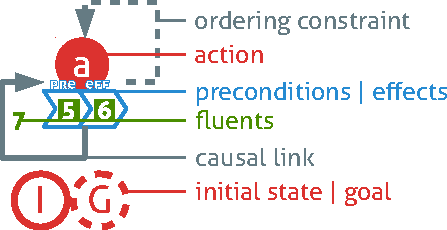
\includegraphics{graphics/legend.pdf}
\caption{Global legend for how partial plans are represented in the
current paper\label{fig:legend}}
\end{figure}

\subsection{Classic planning}\label{classic-planning}

\begin{definition}[Fluents]

A fluent is a property of the world. It is often represented by first
order logical propositions but in our case we choose to focus on the
algorithm and to represent fluents as simple literals (fully
instantiated). We note \(\lnot f\) the complementary fluent of \(f\)
meaning that \(f\) is true when \(\lnot f\) is false and vice-versa.

In order to make our example simpler we use \(\mathbb{Q}^*\), the set of
relative integers without \(0\), as the fluent domain. We use negative
integers to represent opposite fluents.

\end{definition}

\begin{definition}[State]

We define a state as a set of fluents. States can be additively
combined. We note
\(s_1 + s_2 = \left( s_1 \cup s_2 \right) - \left\{ f \middle| f \in s_1 \land \lnot f \in s_2 \right\}\)
such operation. It is the union of the fluents with an erasure of the
complementary ones.

\end{definition}

\begin{definition}[Action]

An action is a state operator. It is represented as a tuple
\(a = \langle pre, eff \rangle\) with \(pre\) and \(eff\) being sets of
fluents, respectively the preconditions and the effects of \(a\). An
action can be used only in a state that verifies its preconditions. We
note \(s \models a \Leftrightarrow pre(a) \subset s\) the verification
of an action \(a\) by a state \(s\).

An action \(a\) can be functionally applied to a state \(s\) following :
\[a:= \substack{ \left\{ s \models a \middle| s \in S\right\} \to S\\
    a(s) \mapsto s + eff(a)}\] with \(S\) being the set of all states.
There are some special names for actions. An action with no
preconditions is synonymous to a state and one with empty effect is
called a goal.

\end{definition}

\subsection{Plan Space Planning}\label{plan-space-planning}

\subsubsection{Problem}\label{problem}

We define a partial plan satisfaction problem as a tuple noted
\(P = \langle A, I, G, p \rangle\) with :

\begin{itemize}
\tightlist
\item
  \(I\) and \(G\) being the pseudo actions representing respectively the
  initial state and the goal.
\item
  \(p\) being a partial plan to refine.
\item
  \(A\) the set of all actions.
\end{itemize}

\begin{definition}[Partial Plan]

A \emph{partial plan} is a tuple \(p = \langle A_p, L\rangle\) where
\(A_p\) is a set of steps (actions) and \(L\) is a set of causal links
of the form \(a_i \xrightarrow{f} a_j\), such that
\(\{ a_i, a_j \} \subset A_p \land f \in eff(a_i) \cap pre(a_j)\) or
said otherwise that \(f\) is provided by \(a_i\) to \(a_j\) via this
causal link. We include the ordering constraints of PSP in the causal
links. An ordering constraint is noted \(a_i \to a_j\) and means that
the plan consider \(a_i\) as a step that is prior to \(a_j\) without
specific cause (usually because of threat resolution).

\end{definition}

\subsubsection{Flaws}\label{flaws}

When refining a partial plan, we need to fix flaws. Those could be
present or be created by the refining process. Flaws can either be
unsatisfied subgoals or threats to causal links.

\begin{definition}[Subgoal]

A subgoal \(s\) is a precondition of an action \(a_s \in A_p\) with
\(s \in pre(a_s)\) that isn't satisfied by any causal link. We can note
a subgoal as :
\[a_i \xrightarrow{s} a_s \notin L \mid \{ a_i, a_s \} \subset A_p \]

A resolver for a subgoal is an action \(a_r \in A\) that has \(s\) as an
effect \(s \in eff(a_r)\). It is inserted along with a causal link noted
\(a_r \xrightarrow{s} a_s\).

\end{definition}

\begin{definition}[Threat]

A step \(a_t\) is said to threaten a causal link
\(a_i \xrightarrow{t} a_j\) if and only if
\[\neg t \in eff(a_t) \land a_i \succ a_t \succ a_j \models L\] Said
otherwise, the action has a possible complementary effect that can be
inserted between two actions needing this fluent while being consistant
with the ordering constraint in \(L\).

The usual resolvers are either \(a_t \to a_i\) or \(a_j \to a_t\) which
are called respectively promotion and demotion links. Another resolver
is called a white knight that is an action \(a_k\) that reestablish
\(t\) after \(a_t\).

\end{definition}

\subsubsection{Solution}\label{solution}

The solution of a PSP problem is a valid partial plan that respect the
specification of said problem (only using actions in \(A\) and having
the correct initial and goal step).

\begin{definition}[Consistency]

A partial plan is consistent if it contains no ordering cycles. That
means that the directed graph formed by step as vertices and causal
links as edges isn't cyclical. This is important to guarantee the
soundness of the algorithm.

\end{definition}

\begin{definition}[Flat Plan]

We can instantiate one or several flat plans from a partial plan. A flat
plan is an ordered sequence of actions \(\pi = [ a_1, a_2 \ldots a_n]\)
that acts like a pseudo action
\(\pi = \langle pre_\pi, eff_\pi \rangle\) and can be applied to a state
\(s\) using functional composition operation
\(\pi := \bigcirc_{i=1}^n a_n\).

We call a flat plan valid if and only if it can be functionally applied
on an empty state. We note that this is different from classic state
planning because in our case the initial state is the first action that
is already included in the plan.

\end{definition}

\begin{definition}[Validity]

A partial plan is valid if and only if it is consistent and if all the
flat plan that can be generated are valid.

\end{definition}

\section{Classical POP}\label{classical-pop}

Partial Order Planning (POP) is a popular implementation of the general
PSP algorithm. It is proven to be sound and complete {[}5{]}. The
completeness of the algorithm guarantees that if the problem has a
solution it will be found by the algorithm. The soundness assures that
any answer from the algorithm is valid. POP refines a partial plan by
trying to fix its flaws.

\subsection{Description}\label{description}

\begin{algorithm}\caption{Classical Partial Order Planning algorithm}\label{pop}\begin{algorithmic}

\Function{pop}{Queue of Flaws $agenda$, Problem $P$}
\State \Call{populate}{$agenda$, $P$} \Comment{Only on first call}
\If{$agenda = \emptyset$} \State \Return Success
\Comment{Stop all recursion} \EndIf
    \State Flaw \(f\gets agenda.pop\)
\Comment{First element of the queue} \State Resolvers \(R \gets\)
\Call{resolvers}{$f$, $P$} \Comment{Ordered list of resolvers to try}
\ForAll{$r \in R$} \Comment{Choice operator}
\State \Call{apply}{$r$, $P.p$} \If{\Call{consistent}{$P.p$}}
\State \Call{pop}{$agenda \cup$ \protect\Call{relatedFlaws}{$f$}, $P$}
\Else 
            \State \Call{revert}{$r$, $P.p$} \EndIf
    \EndFor
    \State \Return Failure \Comment{Return to last choice of resolver}
\EndFunction

\end{algorithmic}\end{algorithm}

From that point the base algorithm is very similar for any
implementation of POP : using an agenda of flaws that is efficiently
updated after each refinement of the plan. A flaw is selected for
resolution and we use a non deterministic choice operator to pick a
resolver for the flaw. The resolver is inserted in the plan and we
recursively call the algorithm on the new plan. On failure we return to
the last non deterministic choice to pick another resolver. The
algorithm ends when the agenda is empty or when there is no more
resolver to pick for a given flaw.

\subsection{Limitations}\label{limitations}

This standard way of doing have seen multiple improvements over
expressiveness like with UCPOP {[}6{]}, hierarchical task network to add
more user control over sub-plans {[}7{]}, cognition with defeasible
reasoning {[}8{]}, or speed with multiple ways to implement the popular
fast forward method from state planning {[}9{]}. However, all these
variants do not treat the problem of online planning, resilience and
soft solving.

Some other closer works like {[}4{]} treats the problem of online
planning by removing big chuncks of the partial plan by identifying
incorect trees in the plan. This causes an heavy replanning of the
problem even if only one action needed removal. This is a big problem
when trying to adapt a plan with minimal changes due to replanning.

Indeed, all these problems can affect POP's performance and quality as
they can interfere with POP's inner working when the algorithm is able
to give an answer at all.

\begin{figure}[htbp]
\centering
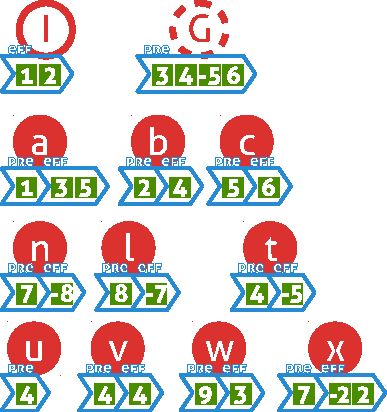
\includegraphics{graphics/problem.pdf}
\caption{A simple problem that will be used throughout this
paper\label{fig:problem}}
\end{figure}

Before continuing, we present a simple example of classical POP
execution with the problem represented in figure \ref{fig:problem}. We
did not represent empty preconditions or effects to improve readability.
Here we have an initial state
\(I = \langle \emptyset , \{ 1, 2 \} \rangle\) and a goal
\(G = \langle \{ 3, 4, -5, 6 \}, \emptyset \rangle\) encoded as dummy
steps. We also introduce actions that are not steps yet but that are
provided by \(A\). The actions \(a\), \(b\) and \(c\) are normal actions
that are useful to achieve the goal. The action \(t\) is meant to be
threatening to the plan's integrity and will generate threats. We
introduce \(u\) as a useless action, \(v\) as a toxic action, \(w\) as a
dead-end action and \(x\) as a contradictory action.

\begin{figure}[htbp]
\centering
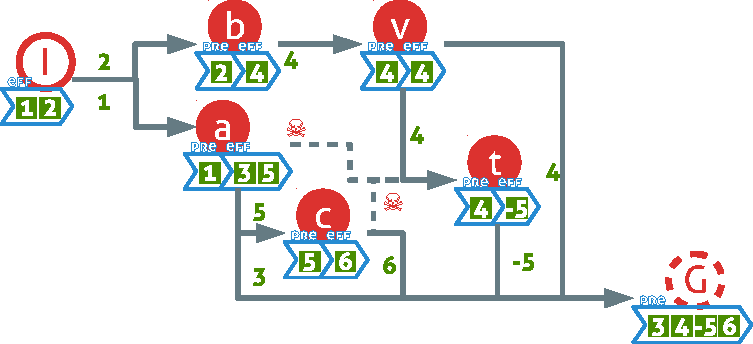
\includegraphics{graphics/pop.pdf}
\caption{Standard POP result to the problem\label{fig:pop}}
\end{figure}

This example has been crafted to illustrate problems with standard POP
implementations. We give a possible resulting plan of standard POP in
figure \ref{fig:pop}. We can see some issues as for how the plan has
been built. The action \(v\) is being used even if it is useless since
\(b\) already provided fluent \(4\). We can also notice that despite
being contradictory the action \(x\) raised no alarm. As for ordering
constraints we can clearly see that the link \(a \to t\) is redundant
with the path \(a \xrightarrow{5} c \to t\) that already puts that
constraint by transitivity. Also some problems arise during execution
with the selection of \(w\) that causes a dead-end.

Of course the flaw selection mechanism of certain variant can prevent
that to happen in that case. But often flaw selection mechanisms are
more speed oriented and will do little if a toxic action seems to fit
better than a more coherent but complex one.

All these issues are caused by what we call \emph{defects} as they are
not regular PSP flaws but they still cause problems with execution and
results. We will address these defects and propose a way to fix them in
\hyperref[defects]{the next section}.

\section{Auxiliary algorithms to POP}\label{auxiliary-algorithms-to-pop}

In order to improve POP algorithms' resilience, online performance and
plan quality, we propose a set of auxiliary algorithms that provides POP
with a clean and efficiently populated initial plan.

\subsection{Proper plan generation}\label{proper-plan-generation}

\begin{algorithm}\caption{Proper plan generation algorithm for a given goal $g$}\label{properplan}\begin{algorithmic}

\Function{properPlan}{Goal $g$, Actions $A$} \State Partial Plan
\(p \gets \emptyset\) \State Actions \(relevants \gets\)
\Call{satisfy}{$g$, $A$, $p$}
\Comment{Satisfy given goal with all necessary actions and causal links}
\State Queue of Actions \(open \gets relevants\)
\While{$open \neq \emptyset$} \State Action \(a\gets open.pop\)
\State Actions \(candidates \gets\) \Call{satisfy}{$a$, $A$, $p$}
\ForAll{$candidate \in candidates$} \If{$candidate \notin relevants$}
\State \(open.push(candidate)\) \EndIf
        \EndFor
    \EndWhile
\EndFunction

\end{algorithmic}\end{algorithm}

As in online planning goals can be known in advance, we add a new
mechanism that generates proper plans for goals. We take advantage of
the fact that this step can be done offline to improve performance for
online planning. This offline execution prevents us to access the
details of the initial state of the world as it will be defined at
runtime. We define for that the concept of \emph{participating action}.
An action \(a \in A\) participates in a goal \(G\) if and only if \(a\)
has an effect \(f\) that is needed to accomplish \(G\) or that is needed
to accomplish another participating action's preconditions. A proper
plan is a partial plan that contains all participating actions as steps
and causal links that bind them with the step they are participating in.
This proper plan is independent from the initial step because we might
not have the initial step at the time of the proper plan generation.

This auxiliary algorithm is therefore used as a caching mechanism for
online planning. The algorithm starts to populate the proper plan with a
quick and incomplete backward chaining.

\hyperdef{}{defects}{\subsection{Defect resolution}\label{defects}}

\begin{algorithm}\caption{Defect resolution algorithm}\label{defectresolution}\begin{algorithmic}

\Function{clean}{Problem $P$} \State \Call{illegal}{$P$}
\State \Call{interfering}{$P$} \EndFunction

\Function{illegal}{Problem $P$}
\State \Call{assert}{$pre(P.I) = \emptyset$}
\State \Call{assert}{$eff(P.G) = \emptyset$}
\State \(P.p.A_p \gets P.p.A_p \cup \{P.I, P.G\}\)
\State \Call{breakCycles}{$P$} \State Actions
\(actions \gets P.A \cup P.p.A_p\) \ForAll{Action $a \in actions$}
\State \Call{inconsistent}{$a$, $P$} \State \Call{toxic}{$a$, $P$}
\EndFor
    \State \Call{liarLinks}{$P$} \EndFunction

\Function{interfering}{Problem $P$} \State \Call{repeating}{$P$}
\State \Call{useless}{$P$} \EndFunction

\end{algorithmic}\end{algorithm}

When the POP algorithm is used to refine a given plan (that was not
generated with POP or that was altered), a set of new defects can be
present in it interfering in the resolution and sometimes making it
impossible to solve. We emphasize that these defects are not regular POP
flaws but new problems that classical POP can't solve. The aim of this
auxiliary algorithm is to clean the plans from such defects in order to
improve computational time, resilience and plan quality . It should be
noted that in some cases cleaning plans will increase the number of
flaws in the plan but will always improve the overall quality of it.

There are two kinds of defects: the illegal defects that violate base
hypothesis of PSP and the interference defects that can lead to
excessive computational time and to poor plan quality.

\begin{definition}[Illegal defects]

These defects are usually hypothesized out by regular models. They are
illegal use of partial plan representation and shouldn't happen under
regular circumstances. They may appear if the input is generated by an
approximate cognitive model that doesn't ensure consistency of the
output or by unchecked corrupted data.

\end{definition}

\begin{definition}[Cycles]

A plan cannot contain cycles as it makes it impossible to complete.
Cycles are usually detected as they are inserted in a plan but poor
input can potentially contains them and breaks the POP algorithm as it
cannot undo cycles.

We use a popular and simple Depth First Search (DFS) algorithm to detect
cycles. Upon cycle detection the algorithm can remove arbitrarily a link
in the cycle to break it. The most effective solution is to remove the
link that is the farthest from the goal travelling backward as it would
be that link that would have been last added in the regular POP
algorithm.

\end{definition}

\begin{definition}[Inconsistent actions]

In a plan some actions can be illegal for POP. Those are the actions
that are contradictory. An action \(a\) is contradictory if and only if
\[\{f, \lnot f \} \in eff(a) \lor \{f, \lnot f \} \in pre(a)\]

We remove only one of those effect or preconditions based on the usage
of the action in the rest of the plan. If none of those are used we
choose to remove both.

\end{definition}

\begin{definition}[Toxic actions]

These actions are those that have effects that are already in their
preconditions. This can damage a plan as well as make the execution of
POP algorithm much longer than necessary. They are defined as :
\[a | pre(a) \cap eff(a) \neq \emptyset\]

This is fixed of one of two ways : if the action has only some of its
fluent toxic (\(pre(a) \nsubseteq eff(a)\)) then the toxic fluents are
removed following \(eff(a) = eff(a)-pre(a)\), otherwise the action is
removed alltogether from plan and \(A\).

\end{definition}

\begin{definition}[Liar links]

The defects can be related to incorrect links. The first of which are
liar links : a link that doesn't reflect the preconditions or effect of
its source and target. We can note
\[a_i \xrightarrow{f} a_j | f \notin eff(a_i) \cap pre(a_j)\]

These can form with the way inconsistent actions are fixed : a deleted
fluent could still have links in the plan .

To resolve the problem we either replace \(f\) with a saviour, i.e.~a
fluent in \(eff(a_i) \cap pre(a_j)\) that isn't already provided, or we
delete the link all together.

\end{definition}

\subsubsection{Interference defects}\label{interference-defects}

This kind of defects is not as toxic as the illegal ones: they won't
make the plan unsolvable but they can still cause performance drops in
POP execution. These can appear more often in regular POP results as
they are not targeted by standard implementations.

\begin{definition}[Redundant links]

This defect can happen in POP generated plans to some extends. A
redundant link have a transitive equivalent of longer length. It means
that a link \(a_i \to a_j\) is redundant if and only if it exists
another path from \(a_i\) to \(a_j\) of length greater to \(1\). Since
POP relies on those additional links, this part focus on removing the
ones that were generated for threat removal purpose to simplify the
plan.

\end{definition}

\begin{definition}[Competing causal links]

Causal links can be found to compete with one another. A competing link
\(a_i \xrightarrow{f} a_k\) competes with another link
\(a_j \xrightarrow{f} a_k\) if it provides the same fluent to the same
action. This cannot happen in classical POP algorithm so it is not
handled by it

In order to prune the least useful actions , we need to remove the least
interesting link. In order to elect the best one , we compare their
respective providing action. We choose the link having the providing
action with the smaller outgoing degree in the planning graph. This
indicates that the action is participating to more other actions. If
both actions have the same outgoing degree then we remove the action
with the most incoming degree . This means that we remove the more needy
action .

\end{definition}

\begin{definition}[Useless actions]

Actions can sometimes have no use in a plan as they don't contribute to
it. It is the case of orphans actions (actions without any links) and .
We also consider useless actions that have no effects (except the goal
step).

\end{definition}

\subsection{Soft resolution}\label{soft-resolution}

\begin{algorithm}\caption{Soft resolution healing algorithm}\label{softresolution}\begin{algorithmic}

\Function{heal}{Problem $P$} \State int \(minViolation \gets \infty\)
\State Plan \(best \gets P.p\) \State Flaw \(annoyer\)
\ForAll{$\langle flaw, plan \rangle \in P.partialSolutions$} \State int
\(currentViolation \gets\) \Call{violation}{$plan$, $P.G$}
\If{$currentViolation < minViolation$} \State \(best \gets plan\)
\State \(annoyer \gets flaw\)
\State \(minViolation \gets currentViolation\) \EndIf
    \EndFor
    \State \(P.p \gets best\)
\State \(P.partialSolutions \gets \emptyset\)
\ForAll{Resolver $resolver \in$ \Call{healers}{$annoyer$}}
\State \Call{apply}{$resolver$, $P.p$} \EndFor
\EndFunction

\end{algorithmic}\end{algorithm}

This auxiliary algorithm is meant to deal with failure. It will heal the
plan to make the failure recoverable for the next iteration of POP. Of
course it can't fix the plan by keeping the problem as it is. This
obviously breaks some properties as the algorithm no longer adheres to
the specification of the input, but in exchange it will always issue a
valid plan whatever happens. For more information on this property go
take a look at the \hyperref[hypersoundness]{appropriate section
bellow}.

Soft failure is useful when the precision and validity of the output is
not the most important criteria we look for. In some cases (like in
recognition processes) it is more useful to have an output even if it is
not exact than no output at all. That is why we propose a soft failing
mechanism for POP algorithms.

\subsubsection{Definitions}\label{definitions-1}

We define first some new notions, then we will explain the healing
algorithm.

\begin{definition}[Needer]

A needer is an action that needs a resolution related to a flaw. We
define different types of needer according to the type of the flaw.

\begin{itemize}
\item
  Subgoal needer For a subgoal \(a_n \xrightarrow{s} a_s\) the needer is
  the action \(a_n\) that has an unsatisfied precondition in the current
  partial plan.
\item
  Threat needer The needer of a threat \(a_t\) of a link
  \(a_p \xrightarrow{t} a_n\) is the target \(a_n\) of the threatened
  causal link.
\end{itemize}

\end{definition}

\begin{definition}[Proper fluents]

A proper fluent of a flaw is the one that caused the flaw. For a subgoal
\(a_n \xrightarrow{s} a_s\) it is the unsatisfied precondition \(s\).
For a threat \(a_t\) of a causal link \(a_p \xrightarrow{t} a_n\) it is
the fluent \(t\) held by the threatened causal link.

\end{definition}

\begin{definition}[Saviour]

The saviour of a flaw is the forged action
\(a_s = \langle \emptyset, \{p\} \rangle | a_s \notin A\) with \(p\)
being the proper fluent of the flaw.

\end{definition}

\begin{definition}[Healers]

The concept of healer is made to target rogue flaws that caused total
failure. A healer is a resolver that is built around the saviour of the
flaw to provide for it . The general formula of a healer is the
following : \[a_s \xrightarrow{p} a_n\] with \(a_s\) being the saviour
of the flaw.

For threats we need an additional healer specified as an ordering
constraint from the threatening action to the saviour \(a_t \to a_s\) to
ensure that the saviour acts after the threat and therefore provides the
proper fluent for the needer.

\end{definition}

\begin{definition}[Violation degree]

The violation degree \(v(p)\) of a plan \(p\) is an indicator of the
health of a partial plan. It is the sum of the number of flaws and the
number of saviours in the plan.

\end{definition}

\subsubsection{Healing process}\label{healing-process}

The healing method is to keep track of reversions in the algorithm by
storing the partial plan and the unsatisfiable flaw each time a non
deterministic choice fails. We note the set of these failed plans \(F\).
As the POP algorithm encounters a final failure, this auxiliary
algorithm get invoked. The aim is to evaluate each backtracking partial
plan to choose the best one.

Therefore we add an order relation for \(F\) noted
\[\prec : p \prec q \iff v(p) < v(q) | \{p, q\} \subset F\]

Once the POP algorithm fails completely the soft failing algorithm can
be invoked to heal the plan. It chooses the best plan
\(b | \forall p \in F, b \prec p\) to heal it. If two plans have the
same violation degree, the algorithm chooses one arbitrarily .

The healing process is similar to how POP works : we apply the healer of
the flaw that caused the failure of the partial plan we chosen. We empty
the set \(F\) to allow POP to iterate further since the flaw is
resolved. The healing process can be done for each unsolved flaws as POP
fails repeatedly. This ensures some interesting properties explained in
the following section.

\section{SODA POP and its properties}\label{soda-pop-and-its-properties}

After defining the way our algorithms work we will focus on the
properties that can be achieved by combining them together.

\begin{algorithm}\caption{Combining all algorithms into SODA POP}\label{soda}\begin{algorithmic}

\Function{soda}{Problem $P$} \State \(P.p \gets\)
\Call{properPlan}{$P.G$, $P.A$} \State \Call{clean}{$P$} \State bool
\(valid \gets false\) \While{$\lnot valid$} \(valid \gets\)
\State \Call{pop}{$P$} \(= Success\) \If{$valid$}
\State \Call{clean}{$P$} \State \Return \(Success\) \EndIf
        \State \Call{heal}{$P$} \EndWhile
\EndFunction

\end{algorithmic}\end{algorithm}

\subsection{Convergence of POP}\label{convergence}

As to our knowledge no proof of the convergence of POP has been done we
want to explicitly formulate one.

The classic planning problem is already proven to be decidable without
functions in the fluents {[}3{]}. Therefore we can categorise the
termination cases. In the case of a solvable problem, POP is proven to
be complete. This ensures convergence in that case. Now for the more
complex case of unsolvable problems we need to refer to the way POP
works. POP algorithm will seek to solve flaws. At any time there is a
finite number of flaws since the plans have a finite number of steps. As
POP resolves these flaws it will either continue until resolution or
until failure. The problem is that POP can encounter loops in the
dependancies of actions or in threats resolution. These loops can't
occur in POP algorithm since a cycle in the ordering constraints
instantly causes a failure as the plan isn't consistent anymore. This
prooves that POP always converges.

\subsection{Hyper soundness}\label{hypersoundeness}

Now that we proved that regular POP converges we can introduce the next
property : hyper soundness. An algorithm is said to be hyper sound when
it gives a valid solution for all problems including unsolvable ones. We
note that this property isn't compatible with consistency regarding the
original problem but still does regarding the derived problem that
includes all fake actions in \(A\).

The hyper soundness of our combined algorithm is proven using the
convergence of POP and the way the Soft solving behaves. As a POP fails
it will issue flawed partial plans. As we fix the flaws artificially we
make sure that this failure won't happen again in the next iteration of
POP on the fixed plan. As the number of flaws is finite and POP
converges, the whole algorithm will converge with all flaws solved
therefore issuing a valid plan.

\subsection{Enhancement for online
planning}\label{enhancement-for-online-planning}

\section{Experimental results}\label{experimental-results}

\section*{Conclusion}\label{conclusion}
\addcontentsline{toc}{section}{Conclusion}

\section*{References}\label{references}
\addcontentsline{toc}{section}{References}

\hyperdef{}{ref-weldux5fintroductionux5f1994}{\label{ref-weldux5fintroductionux5f1994}}
{[}1{]} D. S. Weld, ``An introduction to least commitment planning,''
\emph{AI magazine}, vol. 15, no. 4, p. 27, 1994.

\hyperdef{}{ref-richterux5flamaux5f2011}{\label{ref-richterux5flamaux5f2011}}
{[}2{]} S. Richter, M. Westphal, and M. Helmert, ``LAMA 2008 and 2011,''
in \emph{International Planning Competition}, 2011, pp. 117--124.

\hyperdef{}{ref-ghallabux5fautomatedux5f2004}{\label{ref-ghallabux5fautomatedux5f2004}}
{[}3{]} M. Ghallab, D. S. Nau, and P. Traverso, \emph{Automated
planning: theory and practice}. Amsterdam ; Boston: Elsevier/Morgan
Kaufmann, 2004.

\hyperdef{}{ref-vanux5fderux5fkrogtux5fplanux5f2005}{\label{ref-vanux5fderux5fkrogtux5fplanux5f2005}}
{[}4{]} R. Van Der Krogt and M. De Weerdt, ``Plan Repair as an Extension
of Planning.'' in \emph{ICAPS}, 2005, vol. 5, pp. 161--170.

\hyperdef{}{ref-erolux5fumcp:ux5f1994}{\label{ref-erolux5fumcp:ux5f1994}}
{[}5{]} K. Erol, J. A. Hendler, and D. S. Nau, ``UMCP: A Sound and
Complete Procedure for Hierarchical Task-network Planning.'' in
\emph{AIPS}, 1994, vol. 94, pp. 249--254.

\hyperdef{}{ref-penberthyux5fucpop:ux5f1992}{\label{ref-penberthyux5fucpop:ux5f1992}}
{[}6{]} J. S. Penberthy, D. S. Weld, and others, ``UCPOP: A Sound,
Complete, Partial Order Planner for ADL.'' \emph{Kr}, vol. 92, pp.
103--114, 1992.

\hyperdef{}{ref-bechonux5fhipop:ux5f2014}{\label{ref-bechonux5fhipop:ux5f2014}}
{[}7{]} P. Bechon, M. Barbier, G. Infantes, C. Lesire, and V. Vidal,
``HiPOP: Hierarchical Partial-Order Planning,'' in \emph{STAIRS 2014:
Proceedings of the 7th European Starting AI Researcher Symposium}, 2014,
vol. 264, p. 51.

\hyperdef{}{ref-garciaux5fdefeasibleux5f2008}{\label{ref-garciaux5fdefeasibleux5f2008}}
{[}8{]} D. R. García, A. J. García, and G. R. Simari, ``Defeasible
reasoning and partial order planning,'' in \emph{Foundations of
Information and Knowledge Systems}, Springer, 2008, pp. 311--328.

\hyperdef{}{ref-colesux5fforward-chainingux5f2010}{\label{ref-colesux5fforward-chainingux5f2010}}
{[}9{]} A. J. Coles, A. Coles, M. Fox, and D. Long, ``Forward-Chaining
Partial-Order Planning.'' in \emph{ICAPS}, 2010, pp. 42--49.

\end{document}
